\chapter{設計}
本章では,まずADLoggerシステムの設計概要について述べる.
ついで,システム内の各モジュールについて説明する.

\section{本システムの設計概要}
本研究では,学習に対する動機づけを内在化させるため,ADLoggerシステムを提案する.
ADLoggerは学習時間を記録し,その記録を可視化するiOSアプリケーションである.
本システムのシステム構成図を図~\ref{fig:system}に示す.(リマインドモジュール実装前のシステム構成図なので今後直します)
クライアント側はTODOリスト記録モジュール,ストップウォッチモジュール,リマインドモジュールから成る.

\begin{figure}[tb]
	\begin{center}
	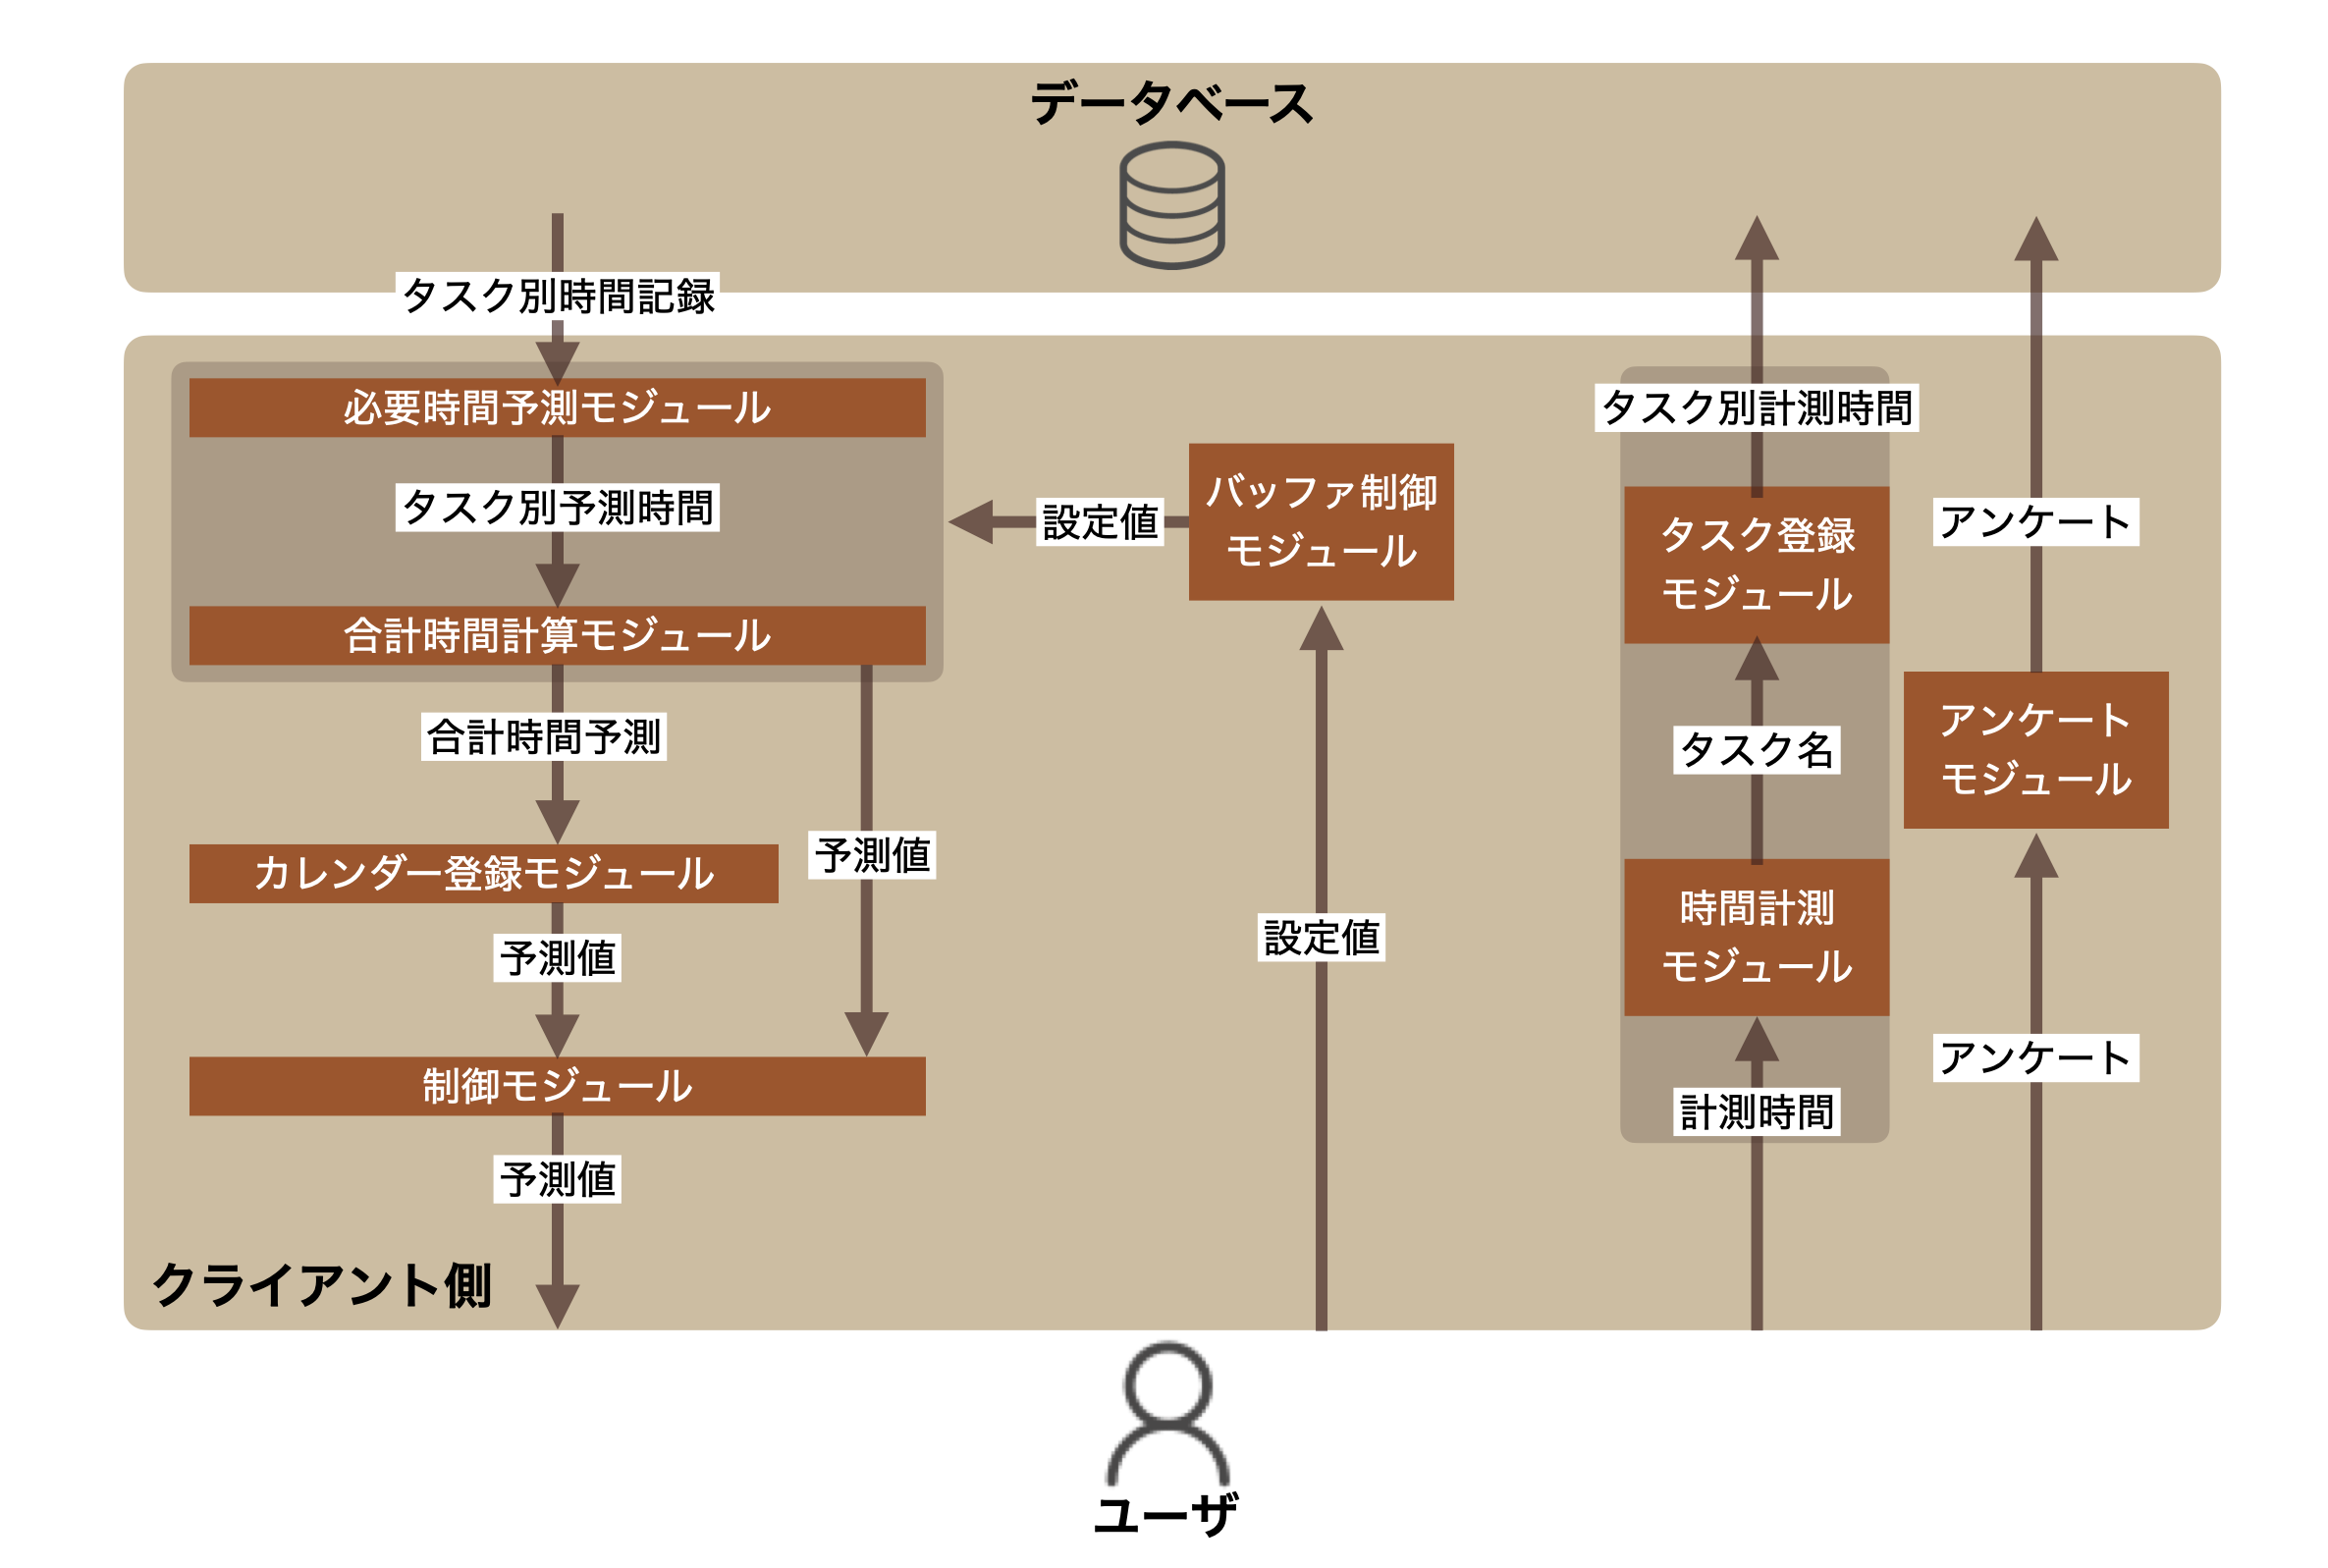
\includegraphics[width=9cm]{images/5/3.png}
	\end{center}
	\caption{システム構成図(暫定版)}
	\label{fig:system}
\end{figure}

\section{クライアント側設計}
本節では,クライアントであるiPhoneアプリケーションを構成するモジュールについて説明する.

\subsection{TODOリスト入力モジュール}
TODOリスト入力モジュールでは,ユーザの日常生活動作を記録する.新規登録で登録を行うと登録順にリストが形成される.TODOカラムは個別に削除が可能である.
\subsection{ストップウォッチモジュール}
TODOリスト内の角日常生活動作カラムの右隣にストップウォッチが表示される.STARTボタンを押すとカウントが始まりSTOPボタンで止まる.TODOリスト外の中央のストップウォッチで準備開始時間から外出時間までを計測する.
\subsection{リマインドモジュール}
実測された時間の開始時刻から出発時刻までの平均を元にリマインドを行う.半分経過時間,及び1/4,3/4経過時間にバイブレーションを鳴らす.
\section{まとめ}
本章では,ADLoggerシステムの設計について述べた.
次章では,本システムの実装について述べる.